\documentclass[12pt,a4paper]{article}
\usepackage[utf8]{inputenc}
\usepackage[T1]{fontenc}
\usepackage[a4paper,top=2.5cm,bottom=2.5cm,left=3cm,right=3cm]{geometry}
\usepackage{graphicx}
\usepackage[justification=default]{subfig}
\usepackage[update]{epstopdf}
\usepackage[labelfont=bf]{caption}
\usepackage[dvipsnames]{xcolor}
\usepackage{fancyhdr}
\usepackage{booktabs}
\usepackage{multicol}
\usepackage{multirow}
\usepackage{titling}
\usepackage{float}
\usepackage{bm}
\usepackage[intlimits]{empheq}
\usepackage[hidelinks]{hyperref}
\usepackage{amsmath}
\usepackage{amssymb}

\usepackage{tikz}
\usetikzlibrary{positioning,3d}


%Bibliography

\usepackage{csquotes}
\usepackage[sorting=none,%
sortcites=true,%
bibencoding=ascii,%
autopunct=true,%
hyperref=true,%
language=auto,%
%backref=true,%
url=false,%
%maxcitenames=10,%
%minbibnames = 20,%
maxbibnames = 3,%
giveninits,
natbib = false,
isbn=false,%
backend=biber]{biblatex}
\addbibresource{bibliography.bib}

\usepackage[]{hyperref}
\usepackage{cleveref}
%%% CREF setup
\crefname{equation}{Eq.}{Eqs.}
\crefname{table}{Table}{Tables}
\crefname{figure}{Fig.}{Figs.}


\begin{document}

\begin{titlingpage}
	\begin{center}
		\begin{figure}
			\centering
			
\includegraphics[width=0.6\textwidth]{figures/logopolimi_mod.jpg}
		\end{figure}
		\Large{\textsc{Politecnico di Milano \\ School of Industrial and Information Engineering \\ Bayesian Learning and Monte Carlo Simulation}}

		\vspace{1cm}

		\rule{0.95\textwidth}{0.7mm}
		{\Large{\textbf{Final project: \\ Yacht Hydrodynamic Resistance}}}
		\rule{0.95\textwidth}{0.7mm}

		\vspace{1cm}

		\large{Authors: \\ \textbf{Peng Rao}}
	\end{center}

\end{titlingpage}

\pagenumbering{roman}

\tableofcontents

\newpage

\setcounter{page}{1}
\pagenumbering{arabic}

\section{Log--log Regression}
\label{sec:loglog}

\subsection{Model and prior}

The physics of slender sailing hulls suggests that, in the bulk regime, the residuary resistance grows as a power of the \textbf{Froude number}, $\mathrm{resistance}\propto Fn^{\,\gamma_F}$ with $\gamma_F$ close to $4$. Taking logarithms turns this multiplicative law into a linear model, in which the exponent appears directly as a regression slope. We therefore fit
\begin{equation}
	\log(\mathrm{resistance})
	= \beta_0 + \beta_F\,\log(\mathrm{Froude})
	+ \sum_{k=1}^{5}\beta_k\,\mathrm{hull}_k + \varepsilon,
	\qquad \varepsilon \sim \mathcal{N}(0,\sigma^2),
	\label{eq:loglog}
\end{equation}
where $\mathrm{hull}_k$ denotes the five geometric form factors. Since the smallest observed resistance is $0.01>0$, the logarithm is well defined for every record and no offset is required. Writing the $n=308$ observations in matrix form as $\bm{y}=\bm{X}\bm{\beta}+\bm{\varepsilon}$ with $\bm{\beta}\in\mathbb{R}^{p}$, $p=7$, we adopt the non-informative \textbf{Jeffreys reference prior}
\begin{equation}
	\pi(\bm{\beta},\sigma^2)\;\propto\;\sigma^{-2},
	\label{eq:prior}
\end{equation}
which lets the data dominate the inference and provides a transparent
Bayesian baseline against which the model-selection and
heteroscedasticity-corrected analyses of the following sections can be
compared.

\subsection{Posterior and Monte Carlo sampling}

Under the prior \eqref{eq:prior} the posterior is Normal--Inverse--Gamma
and is available in closed form. With
$\hat{\bm{\beta}}=(\bm{X}^{\!\top}\bm{X})^{-1}\bm{X}^{\!\top}\bm{y}$ the
least-squares estimate and
$s^2=\lVert \bm{y}-\bm{X}\hat{\bm{\beta}}\rVert^2/(n-p)$ the unbiased error
variance,
\begin{align}
	\sigma^2 \mid \bm{y}           & \sim \text{Inv-Gamma}\!\left(\tfrac{n-p}{2},\,
	\tfrac{(n-p)s^2}{2}\right), \label{eq:post_sigma}                               \\
	\bm{\beta}\mid \sigma^2,\bm{y} & \sim
	\mathcal{N}\!\left(\hat{\bm{\beta}},\,
	             \sigma^2\,(\bm{X}^{\!\top}\bm{X})^{-1}\right). \label{eq:post_beta}
\end{align}
We sample the joint posterior by Monte Carlo: for each of
$M=20{,}000$ iterations we first draw $\sigma^2$ from
\eqref{eq:post_sigma} via a scaled inverse-$\chi^2$ variate and then draw
$\bm{\beta}$ from the Gaussian \eqref{eq:post_beta}. The resulting sample
$\{\bm{\beta}^{(m)},\sigma^{2(m)}\}_{m=1}^{M}$ marginalises the regression
coefficients over $\sigma^2$ (a multivariate Student-$t$) and is used to
obtain all posterior means, standard deviations and $95\%$ credible
intervals, as well as the credible band of the fitted curve.

\subsection{Results}

\Cref{tab:loglog} (in the appendix) reports the posterior summaries. The model explains the
data very well ($R^2=0.97$, residual standard deviation $s=0.32$ on the
log scale). The posterior of the Froude exponent is sharply concentrated,
\[
	\beta_F \approx 4.69, \qquad
	95\%\ \text{CI} = [4.60,\ 4.78],
\]
confirming the expected power-law behaviour
$\mathrm{resistance}\sim Fn^{\,4}$ and verifying the project requirement
$\hat\beta_F\approx 4$. \Cref{fig:loglog} (left) shows the log--log
scatter with the posterior-mean line and its $95\%$ credible band: the
band is extremely tight, reflecting the $300$ observations and the strong
signal of the Froude number. The Monte Carlo posterior of $\beta_F$ is
displayed in \cref{fig:loglog} (right); the whole posterior mass sits
above the nominal value $4$ ($\Pr(\beta_F>4\mid\bm{y})\approx 1$), so the
empirical exponent is best described as \emph{slightly steeper} than the
textbook value of four.

\begin{figure}[H]
	\centering
	\subfloat[Power-law fit on log--log axes.]{%
		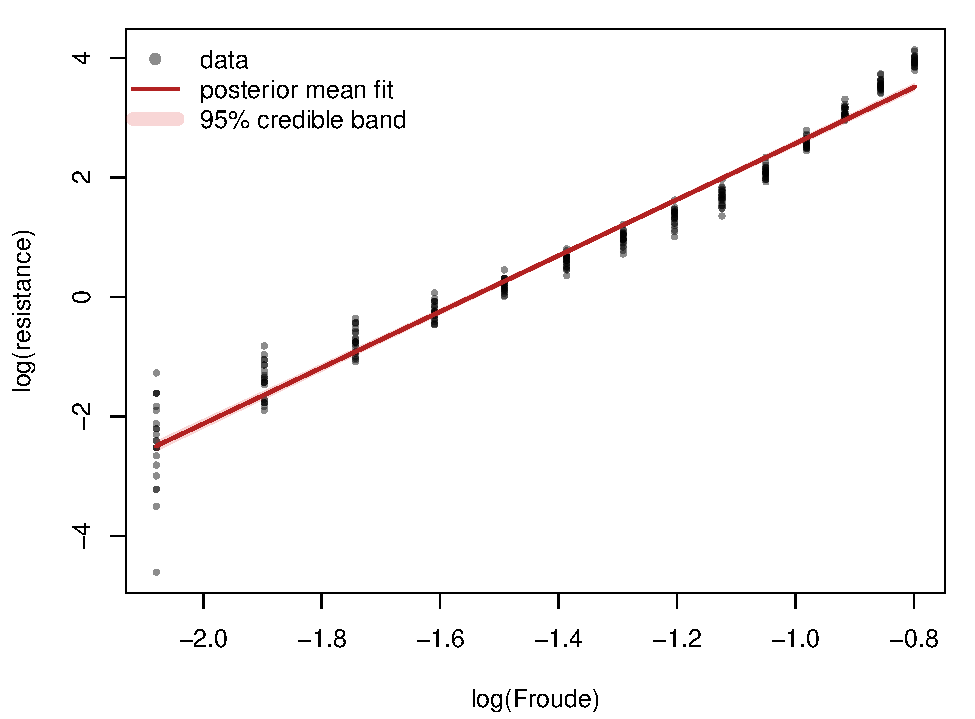
\includegraphics[width=0.49\textwidth]{figures/loglog_scatter.pdf}}
	\hfill
	\subfloat[Monte Carlo posterior of $\beta_F$.]{%
		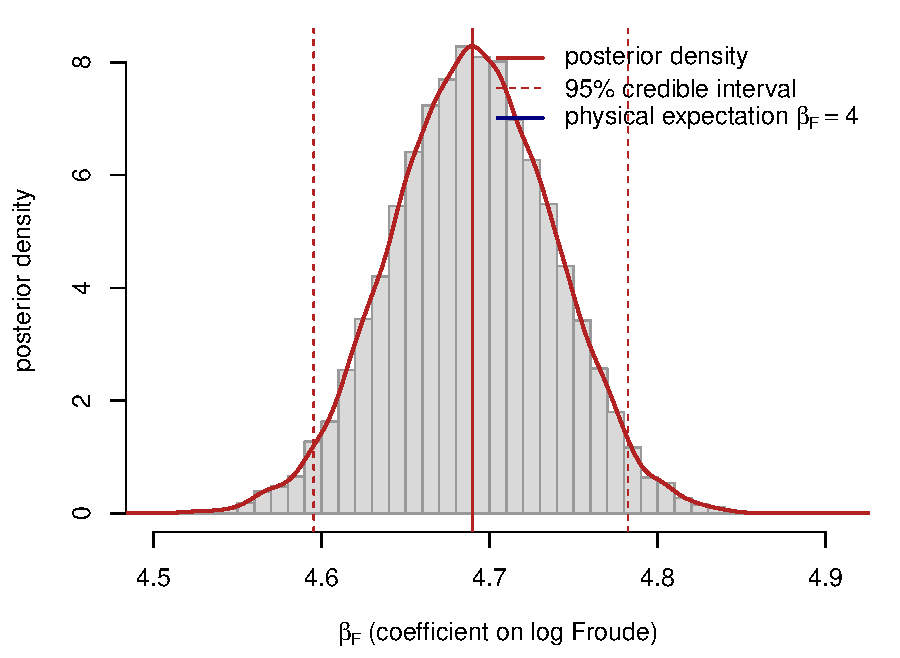
\includegraphics[width=0.49\textwidth]{figures/posterior_betaF.pdf}}
	\caption{Left: observed $\log(\mathrm{resistance})$ against
		$\log(\mathrm{Froude})$ with the posterior-mean regression line (hull
		covariates held at their means) and its $95\%$ credible band. Right:
		Monte Carlo posterior density of the Froude exponent $\beta_F$; the
		dashed lines mark the $95\%$ credible interval and the solid blue line
		the physical reference value $\beta_F=4$.}
	\label{fig:loglog}
\end{figure}

\paragraph{Hull-geometry covariates.}
Once the Froude number is in the model, none of the five hull form factors
is individually credible: every $95\%$ interval comfortably contains zero
(\cref{tab:loglog} and \cref{fig:forest}). The \texttt{prismatic}
coefficient is especially poorly identified, with a posterior standard
deviation of about $1.6$, because the form factors vary only across the
$22$ hulls and are strongly collinear. This near-redundancy is precisely
what the Bayesian model selection of the next section (BAS/BMA over the
$2^5$ submodels) is meant to resolve, by quantifying which covariates
carry signal through their posterior inclusion probabilities rather than
through single-model $p$-values.

\paragraph{Residual diagnostics.}
Although the global fit is excellent, the residuals reveal two systematic
defects that the simple log--log model cannot capture
(\cref{fig:resid}). First, the residuals-versus-fitted panel shows a clear
$\cup$-shaped pattern: a single constant exponent slightly over-predicts
at intermediate speeds and under-predicts at the highest speeds,
consistent with the local Froude exponent increasing from $\approx4.7$ in
the full range to above $6$ in the high-speed subset. Second, the spread
of the residuals is markedly larger at low fitted values, i.e.\ at low
Froude numbers where the resistance is tiny and dominated by measurement
noise --- a textbook signature of heteroscedasticity, also visible as the
fanning of the data cloud on the left of \cref{fig:loglog}. The
Normal Q--Q plot confirms heavier-than-Gaussian lower tails. These two
findings (speed-dependent curvature and non-constant variance) directly
motivate the heteroscedasticity-corrected nonlinear model developed in the
subsequent section.

\begin{figure}[H]
	\centering
	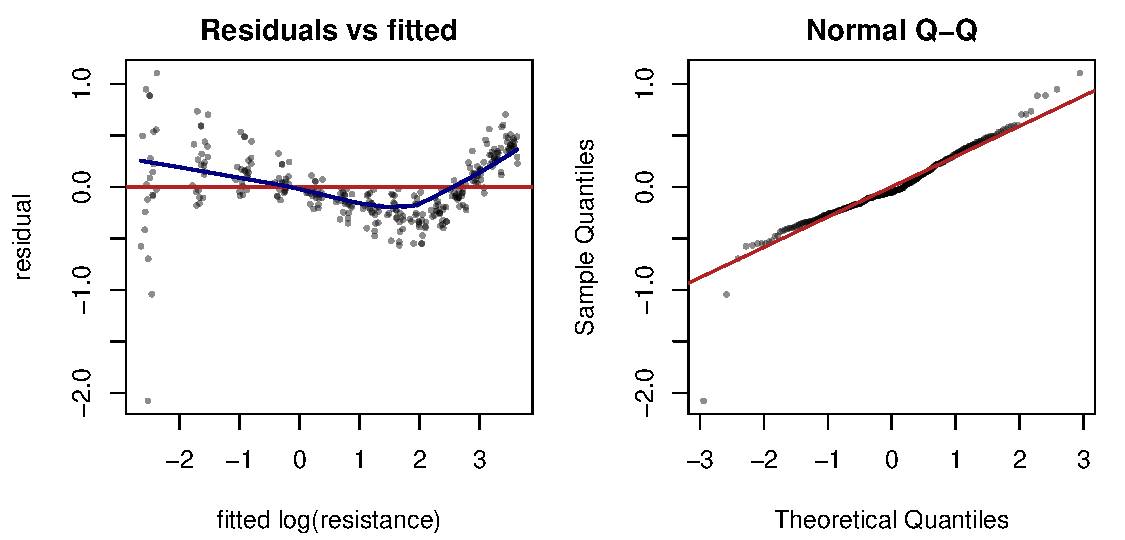
\includegraphics[width=0.95\textwidth]{figures/residual_diag.pdf}
	\caption{Residual diagnostics for the log--log model. Left: residuals
		versus fitted values, with a LOWESS trend (blue) revealing
		speed-dependent curvature and a variance that shrinks as the fitted
		value grows. Right: Normal Q--Q plot, showing heavier-than-Gaussian
		lower tails.}
	\label{fig:resid}
\end{figure}

\begin{figure}[H]
	\centering
	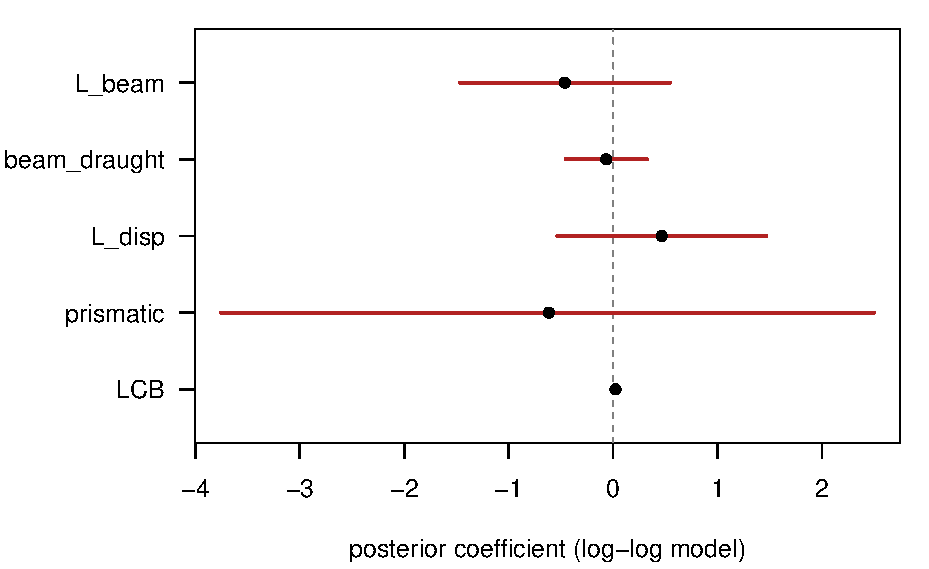
\includegraphics[width=0.7\textwidth]{figures/coef_forest.pdf}
	\caption{Posterior means and $95\%$ credible intervals of the five
		hull-geometry coefficients in the log--log model. Every interval
		straddles zero (dashed line), indicating that no single form factor is
		resolved once the Froude number is accounted for.}
	\label{fig:forest}
\end{figure}

\subsection{Robustness to an informative prior}
\label{sec:informative}

The reference prior \eqref{eq:prior} is deliberately objective: it lets the
data alone estimate the Froude exponent, which we then \emph{verify} against
the physical value $4$. A complementary, fully Bayesian alternative is to
\emph{encode} the physics directly through an informative prior on the
exponent,
\begin{equation}
	\beta_F \sim \mathcal{N}(4,\tau^2),
	\label{eq:inf_prior}
\end{equation}
while keeping the remaining coefficients and $\sigma^2$ vague. The prior
standard deviation $\tau$ controls how strongly the prior insists on the
textbook value. Because the resulting full conditionals remain in closed
form --- $\bm{\beta}\mid\sigma^2,\bm{y}$ Gaussian and
$\sigma^2\mid\bm{\beta},\bm{y}$ Inverse-Gamma --- the posterior is obtained
with a short Gibbs sampler, and we sweep $\tau\in\{0.05,0.1,0.2,0.5\}$.

\Cref{tab:informative} and \cref{fig:informative} summarise the effect. With
a diffuse prior the analysis reproduces the reference result
($\beta_F\approx4.69$). As the prior is tightened around $4$ the posterior
mean is pulled downwards, but the data resist: only a near-dogmatic prior
($\tau=0.05$, a prior $95\%$ interval of roughly $[3.9,4.1]$) drags the
posterior mean as far as $4.33$, and even then
$\Pr(\beta_F>4\mid\bm{y})=1$. For any moderately diffuse physical prior
($\tau\ge0.1$) the likelihood dominates and the posterior stays in the range
$4.56$--$4.69$. The conclusion that the empirical exponent is genuinely
steeper than $Fn^{\,4}$ is therefore \textbf{robust to the prior}: it is a
feature of the $n=308$ observations rather than an artefact of the
non-informative choice. Equivalently, this is a transparent instance of
prior--data conflict, in which a sufficiently informative likelihood
overwhelms all but an unreasonably confident prior.

\begin{table}[H]
	\centering
	\caption{Posterior of the Froude exponent $\beta_F$ under an informative
		prior $\mathcal{N}(4,\tau^2)$ of increasing strength, obtained by Gibbs
		sampling, compared with the reference-prior result.}
	\label{tab:informative}
	\begin{tabular}{l r r r r}
		\toprule
		\textbf{Prior on $\beta_F$} & \textbf{Mean} & \textbf{2.5\%} & \textbf{97.5\%} & $\Pr(\beta_F>4)$ \\
		\midrule
		$\mathcal{N}(4,0.05^2)$     & $4.33$        & $4.26$         & $4.41$          & $1.00$           \\
		$\mathcal{N}(4,0.10^2)$     & $4.56$        & $4.47$         & $4.64$          & $1.00$           \\
		$\mathcal{N}(4,0.20^2)$     & $4.65$        & $4.56$         & $4.74$          & $1.00$           \\
		$\mathcal{N}(4,0.50^2)$     & $4.68$        & $4.59$         & $4.78$          & $1.00$           \\
		\midrule
		reference $\;\sigma^{-2}$   & $4.69$        & $4.60$         & $4.78$          & $1.00$           \\
		\bottomrule
	\end{tabular}
\end{table}

\begin{figure}[H]
	\centering
	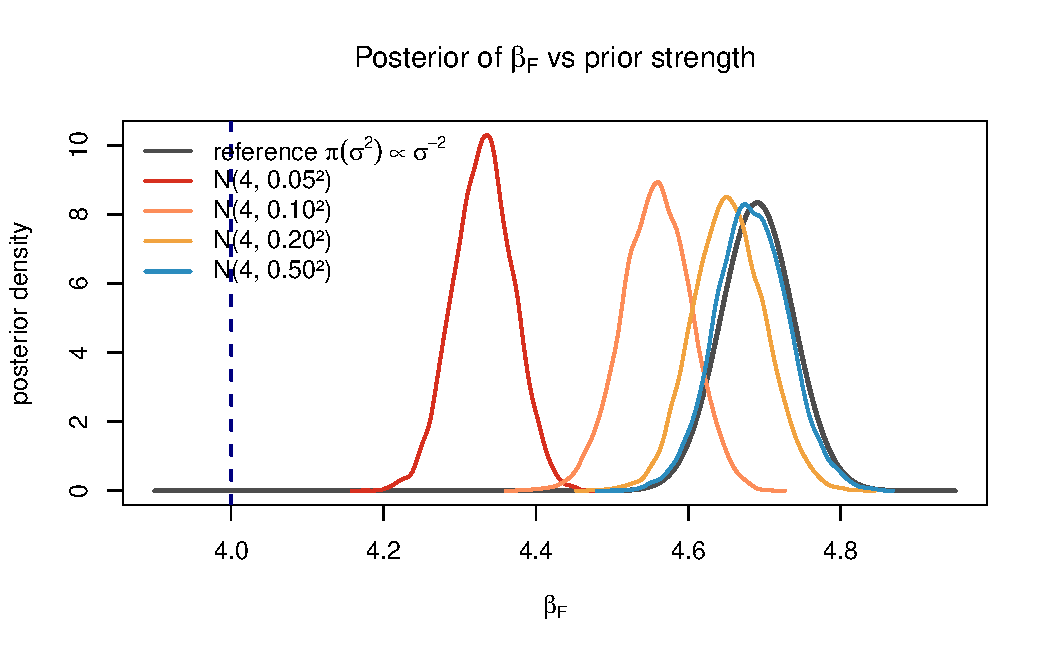
\includegraphics[width=0.72\textwidth]{figures/posterior_betaF_prior.pdf}
	\caption{Posterior density of the Froude exponent $\beta_F$ under
		informative priors $\mathcal{N}(4,\tau^2)$ of increasing strength
		(coloured) and under the reference prior (grey). The dashed blue line
		marks the physical value $\beta_F=4$. Tightening the prior toward $4$
		shifts the posterior only modestly; the data keep it well above $4$
		unless the prior is unreasonably confident.}
	\label{fig:informative}
\end{figure}

\newpage

\section{BAS}

\newpage

\section{Heteroscedasticity-Corrected Nonlinear Model}

\clearpage
\printbibliography[heading=bibintoc, title = {References}]

\clearpage
\appendix
\section{Tables}
\label{app:tables}

\begin{table}[H]
	\centering
	\caption{Variables of the yacht hydrodynamics dataset.}
	\label{tab:variables}
	\begin{tabular}{l l}
		\toprule
		\textbf{Variable}      & \textbf{Description}                                 \\
		\midrule
		\texttt{LCB}           & Longitudinal position of the centre of buoyancy      \\
		\texttt{prismatic}     & Prismatic coefficient                                \\
		\texttt{L\_disp}       & Length--displacement ratio                           \\
		\texttt{beam\_draught} & Beam--draught ratio                                  \\
		\texttt{L\_beam}       & Length--beam ratio                                   \\
		\texttt{Froude}        & Froude number, $Fn = v/\sqrt{gL}$                    \\
		\midrule
		\texttt{resistance}    & Residuary resistance per unit weight of displacement \\
		\bottomrule
	\end{tabular}
\end{table}

\begin{table}[H]
	\centering
	\caption{Posterior summary of the log--log model \eqref{eq:loglog}
		under the reference prior ($M=20{,}000$ Monte Carlo draws). $\Pr(>0)$
		is the posterior probability that the coefficient is positive.}
	\label{tab:loglog}
	\begin{tabular}{l r r r r r}
		\toprule
		\textbf{Coefficient}              & \textbf{Mean} & \textbf{SD} & \textbf{2.5\%} & \textbf{97.5\%} & $\Pr(>0)$ \\
		\midrule
		Intercept $\beta_0$               & $7.183$       & $0.977$     & $5.245$        & $9.122$         & $1.00$    \\
		$\log(\mathrm{Froude})$ $\beta_F$ & $4.690$       & $0.048$     & $4.595$        & $4.782$         & $1.00$    \\
		\texttt{LCB}                      & $0.021$       & $0.012$     & $-0.003$       & $0.046$         & $0.96$    \\
		\texttt{prismatic}                & $-0.616$      & $1.597$     & $-3.753$       & $2.495$         & $0.35$    \\
		\texttt{L\_disp}                  & $0.464$       & $0.512$     & $-0.536$       & $1.466$         & $0.82$    \\
		\texttt{beam\_draught}            & $-0.067$      & $0.200$     & $-0.455$       & $0.324$         & $0.37$    \\
		\texttt{L\_beam}                  & $-0.464$      & $0.515$     & $-1.466$       & $0.542$         & $0.18$    \\
		\bottomrule
	\end{tabular}
\end{table}

\end{document}
